% Created 2022-06-09 do 23:55
% Intended LaTeX compiler: pdflatex
\documentclass[11pt]{article}
\usepackage[utf8]{inputenc}
\usepackage[T1]{fontenc}
\usepackage{graphicx}
\usepackage{grffile}
\usepackage{longtable}
\usepackage{wrapfig}
\usepackage{rotating}
\usepackage[normalem]{ulem}
\usepackage{amsmath}
\usepackage{textcomp}
\usepackage{amssymb}
\usepackage{capt-of}
\usepackage{hyperref}
\author{Massimiliano Falzari (s3459101)}
\date{\today}
\title{Uncertainty in Machine Learning $\backslash$\ Assignment 2}
\hypersetup{
 pdfauthor={Massimiliano Falzari (s3459101)},
 pdftitle={Uncertainty in Machine Learning $\backslash$\ Assignment 2},
 pdfkeywords={},
 pdfsubject={},
 pdfcreator={Emacs 26.3 (Org mode 9.1.9)},
 pdflang={English}}
\begin{document}

\maketitle
\tableofcontents

\section{Is the ELBO a proper scoring rule?}
\label{sec:org84d28b2}
Yes, the ELBO is a proper scoring rule.
By definition a proper scoring rule has the following property:
$$S(p_{\theta},q) <= S(q,q)$$
With equality only holding with \(p_{\theta}(y|x) = q(y|x)\).

We know that the KL-divergence can be used as a scoring rule if we
define it as follows:
$$S(p_{\theta},q) = -D_{KL}(p_{\theta},q)$$
we know that the KL-divergence is always non-negative and
\(D_{KL}(p,q)=0\) iff \(p=q\)
Therefore it satisfies the aforementioned property

Finally, we can rewrite the problem of minimizing the KL-divergence as
maximizing the ELBO. (derivation in the slides)

Therefore, the ELBO is equivalent to the - KL-divergence up to
a constant which means that it is a proper scoring rule.
\section{Disentanglement Applications}
\label{sec:orgbeb721f}
\begin{itemize}
\item Spam detection
\end{itemize}


In this case, in order to decide whether it is spam or not, we only
want to focus on epistemic uncertainty, and we want to remove the
aleatoric uncertainty. It is a case of anomaly detection.

\begin{itemize}
\item Forecasting/Planning
\end{itemize}


When performing forecasting/planning, it can be quite important to
distinguish between epistemic and aleatoric uncertainty. In
particular, it can be useful because we can decide how to weight
these two types of uncertainty. For example, let's say we have two or more
predictions/forecasts/plans with the same total
uncertainty. In this case, it can be crucial to distinguish between
aleatoric and epistemic uncertainty. We probably want to favour plans
that have high aleatoric uncertainty as opposed to high epistemic
uncertainty (Note we are at inference time).


\section{Programming Disentangling Uncertainty}
\label{sec:org309bfc6}
I have used an Ensemble as an uncertainty quantification method.
In particular, a 5-network ensemble was used.
As we can see the domain of the training data is roughly between 0.5
and -0.5 mean while the testing domain is roughly between 1 and
-1.
This was done in order to verify whether the epistemic uncertainty
will increase or not outside of the training domain.
As we can see from Figure 5, after we go outside of the training
domain, the epistemic uncertainty is higher than when we are inside
the training domain. Therefore, this shows that the estimate seems
reasonable (Even though, I expected a higher value).

For the aleatoric uncertainty, on the other hand, (Figure 4) the
network failed to fit the function we used as noise. It almost looks
like the noise is fixed and is not based on the input. That said, even
though the shape of the noise function was not captured, the value
seems to be in line with the mean of the function which is roughly
0.5.

Lastly, we can see that the predicted values as a similar behaviour of
the epistemic uncertainty. In particular, the more we go outside of
the training domain, the more the predicted values does not follow the
function we wanted to fit.(Figure 3)

Finally, the implementation used the DeepEnsembleRegressor from the
keras\(_{\text{uncertainty}}\) library. Generally, an ensemble is simply a set of
networks that are trained on the same data. At inference time (this
was the main feature used from the library) the ensemble estimates
from each of the networks the mean and variance predicted and it
returns the mean of the means and the mean of the variance. In our
case, we used the flag disentangle\(_{\text{uncertainty}}\)= True which instead of
returning the mean and variance of the ensemble returns the
standard deviation of the means for the epistemic uncertainty and the
mean of the standard deviation for the aleatoric uncertainty. These
were the main features used from the library.

\begin{figure}[htbp]
\centering
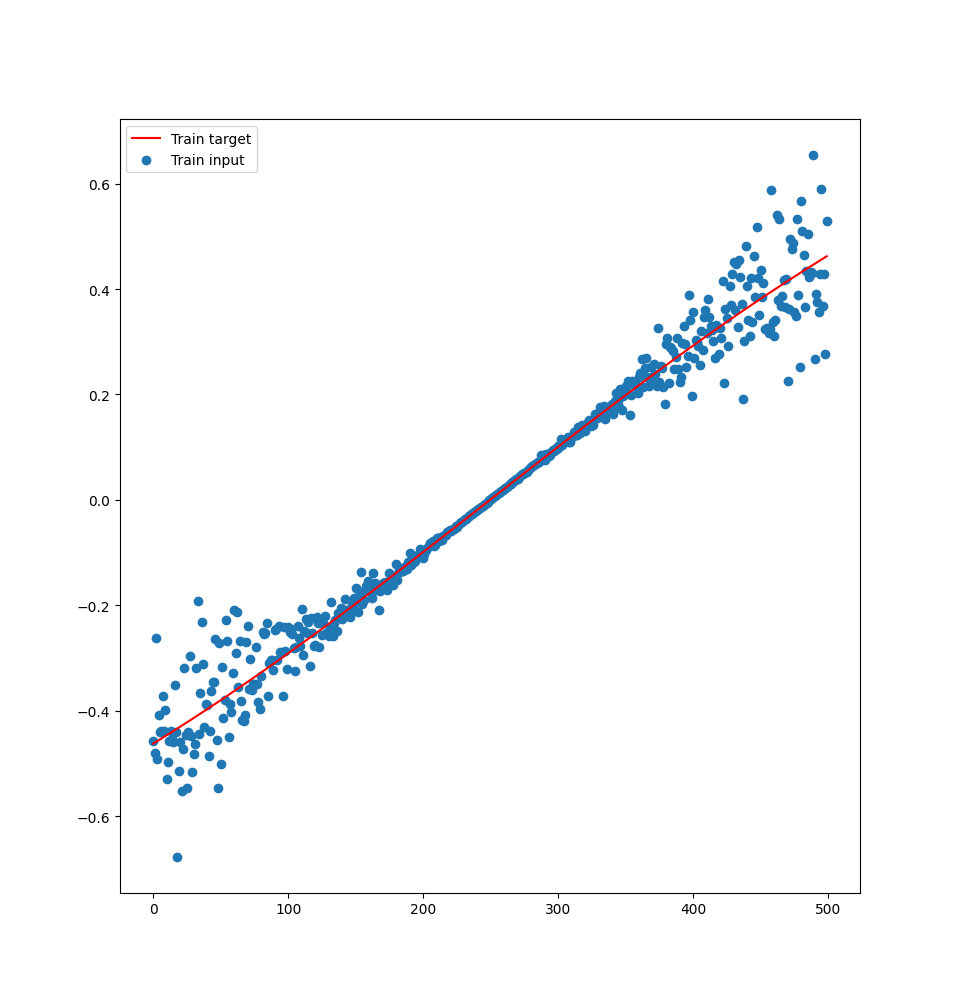
\includegraphics[width=.9\linewidth]{./train.png}
\caption{training data}
\end{figure}
\begin{figure}[htbp]
\centering
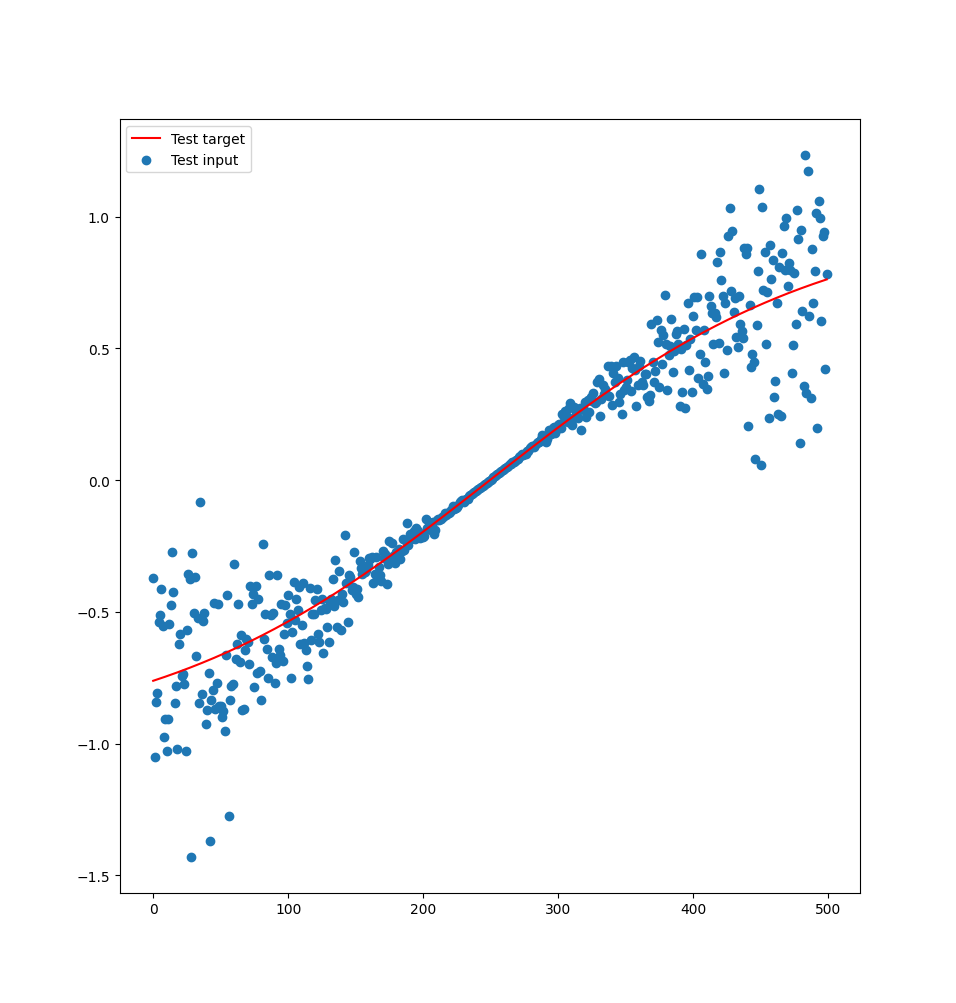
\includegraphics[width=.9\linewidth]{./test.png}
\caption{testing data}
\end{figure}
\begin{figure}[htbp]
\centering
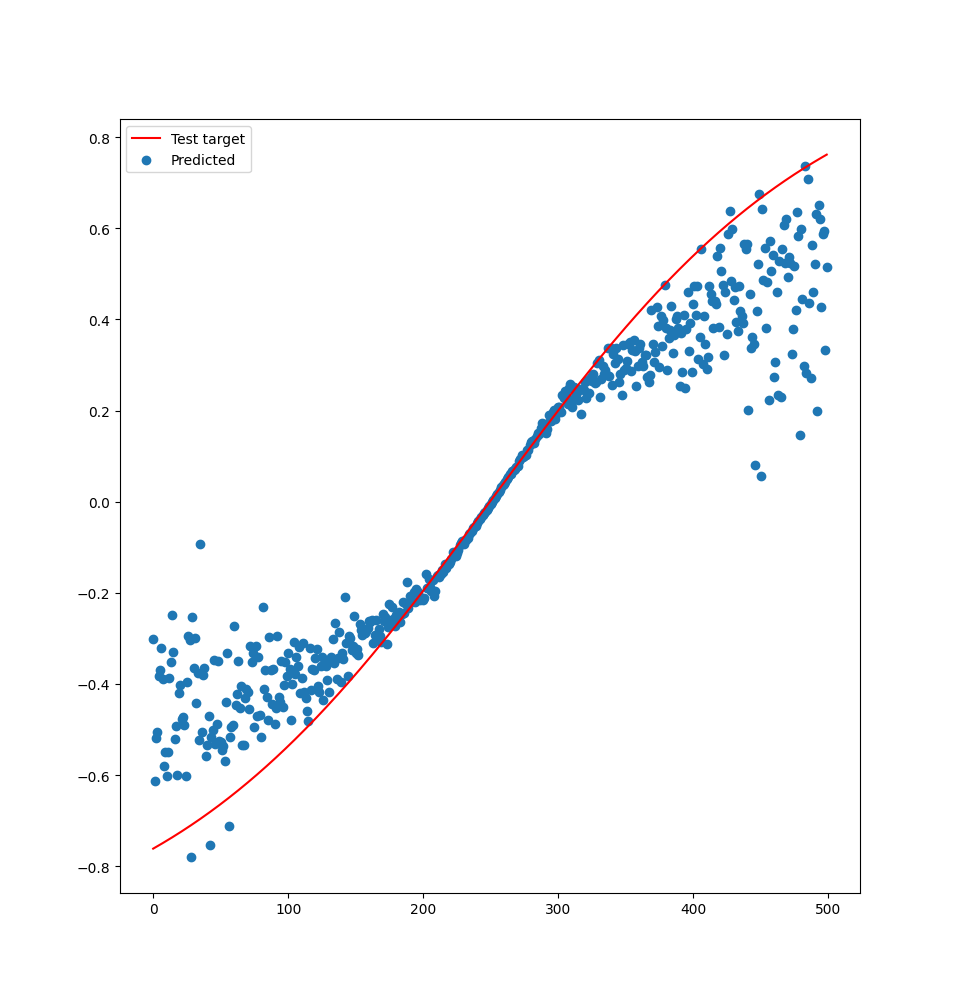
\includegraphics[width=.9\linewidth]{./predicted.png}
\caption{predicted}
\end{figure}
\begin{figure}[htbp]
\centering
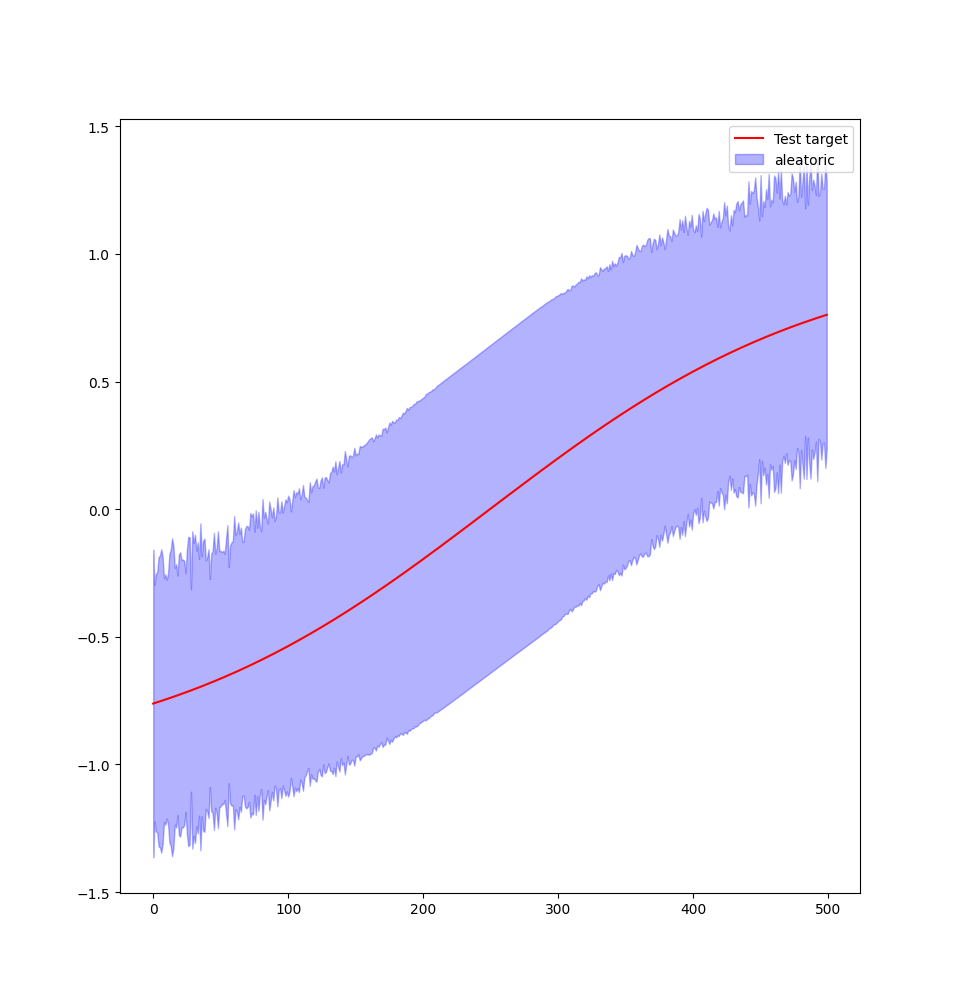
\includegraphics[width=.9\linewidth]{./aleatoric.png}
\caption{aleatoric uncertainty}
\end{figure}
\begin{figure}[htbp]
\centering
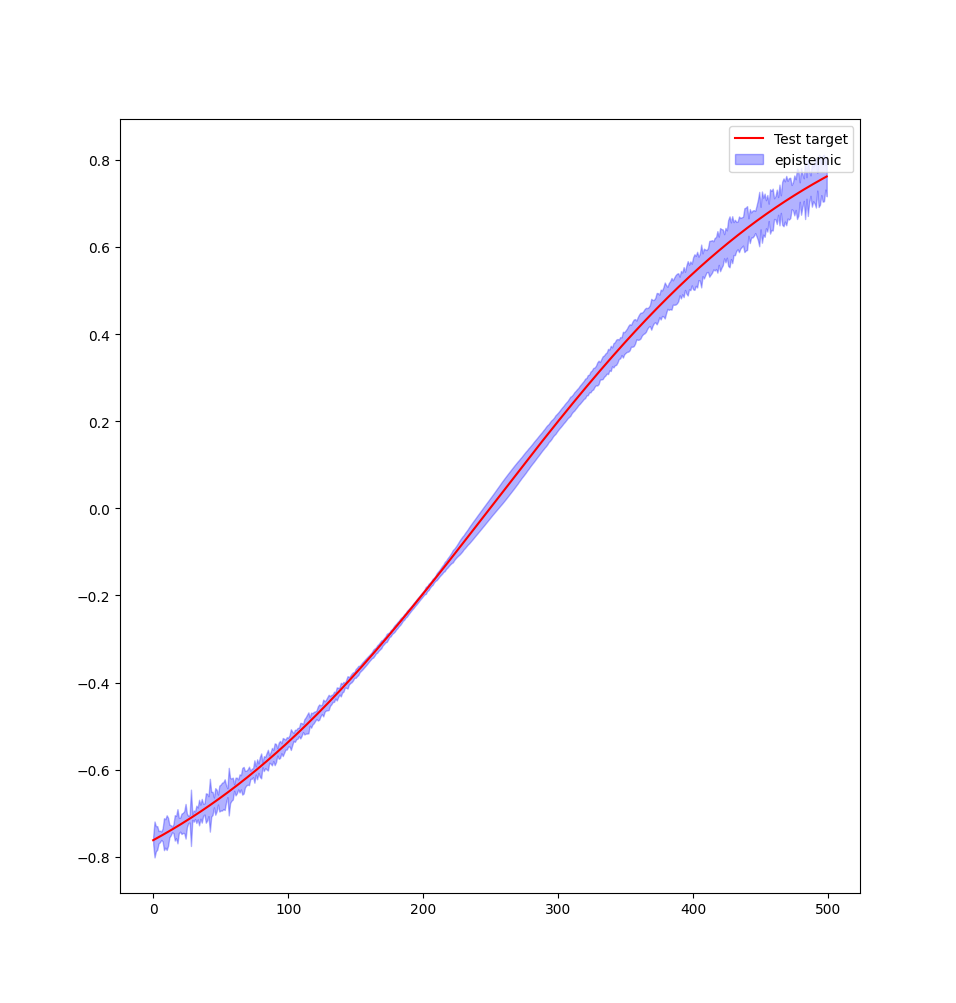
\includegraphics[width=.9\linewidth]{./epistemic.png}
\caption{epistemic uncertainty}
\end{figure}
\end{document}
